\chapter{Software-Entwurf} \label{cha:swentwurf}

\section{Blockansicht}

Im folgenden ist die Struktur (\textit{High-Level-Ansicht}) des Software-Systems in Form eines Blackbox-Diagrams dargestellt.

\begin{figure}[H]
    \centering
    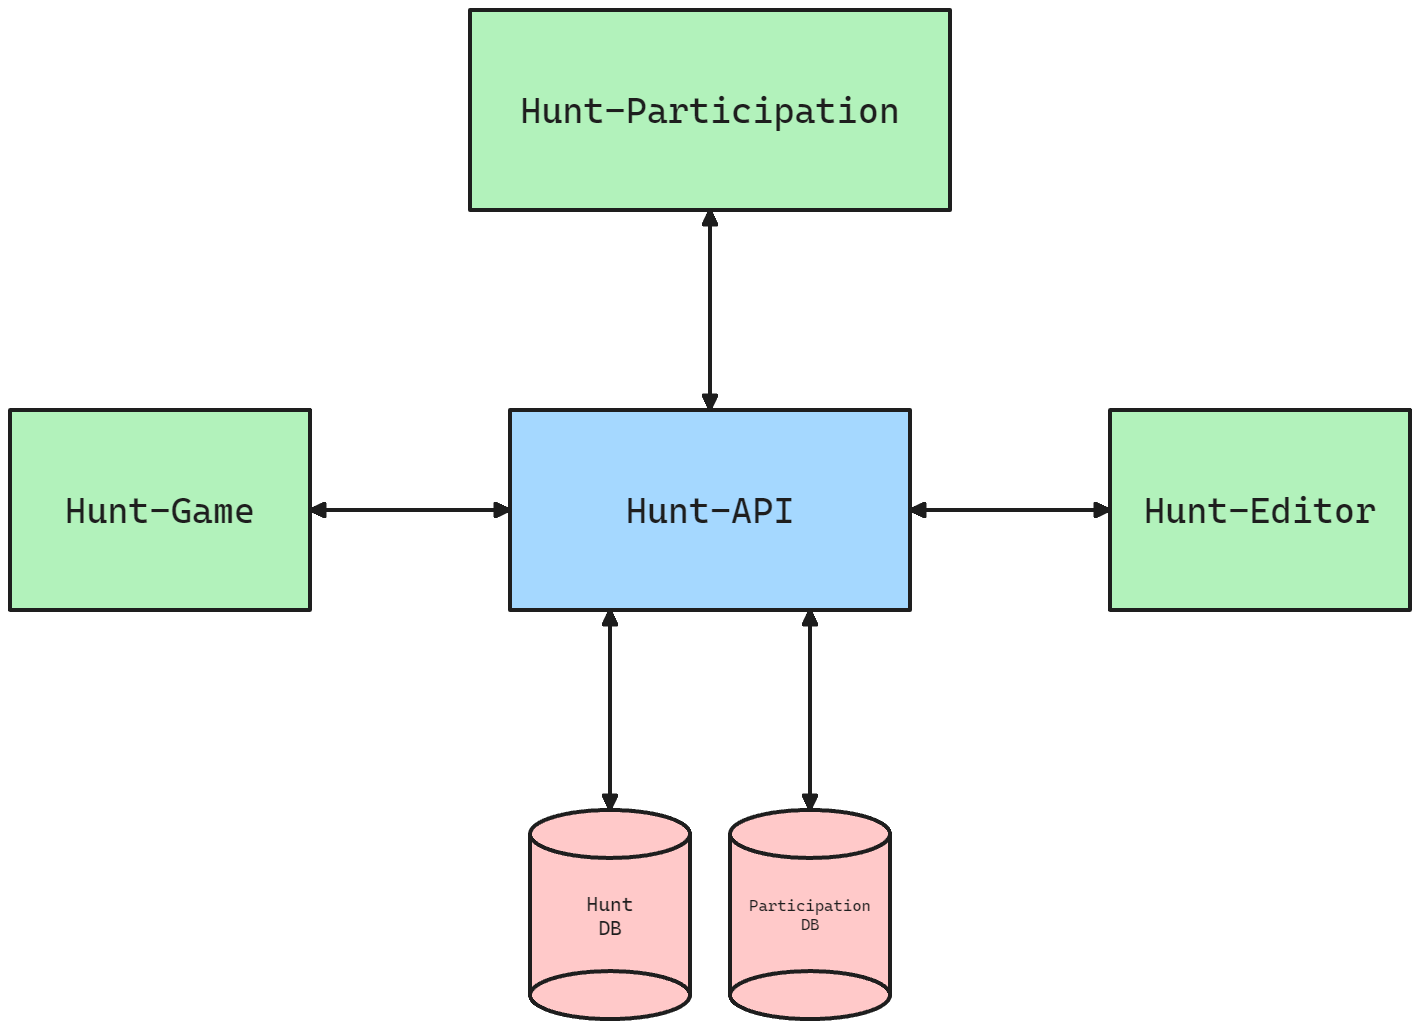
\includegraphics[width=\textwidth]{images/PrAr-Software-Entwurf-Blockansicht.png}
    \caption{Bild Systemkontext als Blackbox-Diagram}
    \label{fig:swentwurf:blackbox}
\end{figure}

Das in Abbildung \ref{fig:swentwurf:blackbox} dargestellte Blackbox-Diagramm beschreibt den Zusammenhang der unterschiedlichen Subsysteme zueinander. Die verschiedenen Aufgaben, die das System zu leisten hat, wurden als einzelne Anwendungen vorhergesehen. Diese sind in Abbildung \ref{fig:swentwurf:blackbox} grün markiert. Dies ermöglicht eine klare Trennung der verschiedenen Domänen (Erstellung, Anmeldung, Durchführung). Das Backend steht als zentrale Schnittstelle für die Bereitstellung systemspezifischer Funktionalitäten zur Verfügung. Dieses sind in Abbildung \ref{fig:swentwurf:blackbox} blau markiert. Für die Datenpersistierung besitzt das Backend zwei Datenbank-Verbindungen. Dieses sind in Abbildung \ref{fig:swentwurf:blackbox} rot markiert.

\section{Hunt-Api Backend} \label{cha:swentwurf:backend}

\subsection{Übersicht}

Anhand einer zentral zur Verfügung stehenden Schnittstelle \textit{Hunt-Api} können die verschiedenen Anwendungen zur Gesamt-Funktionalität des Systems beitragen. Die Schnittstelle bietet verschiedene Endpunkte für die Verwaltung von Schnitzeljagden, Teilnahmen und die bewältigten Aufgaben der Teilnehmer. Eine Darstellung der Hunt-Api Architektur ist in Abbildung \ref{fig:swentwurf:huntapi:subsystem} näher beschrieben.

\begin{figure}[H]
    \centering
    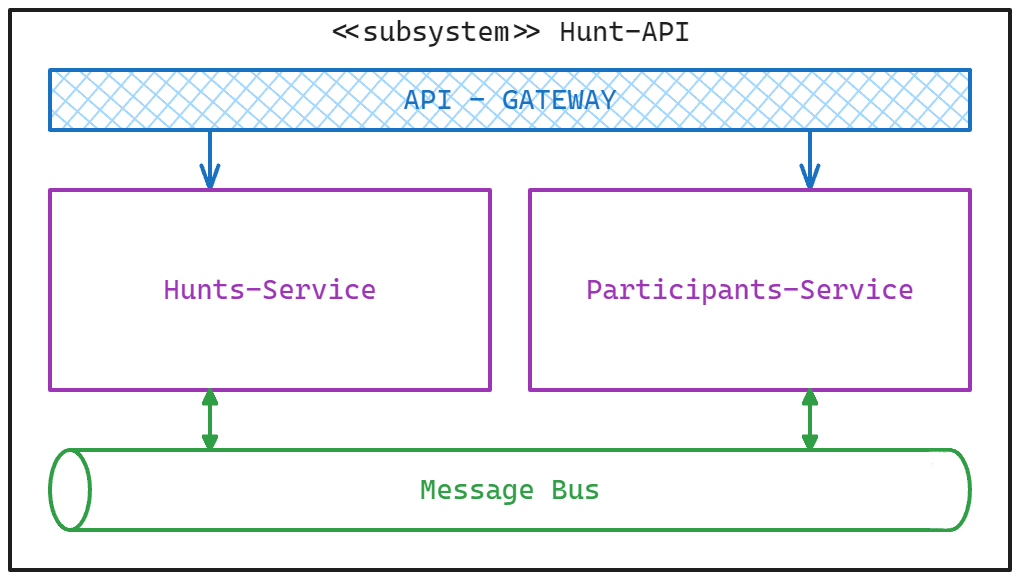
\includegraphics[width=\textwidth]{images/PrAr-Software-Entwurf-Hunt-Api-Subsystem.png}
    \caption{Bild Hunt-Api Subsystem}
    \label{fig:swentwurf:huntapi:subsystem}
\end{figure}

Als Architekturmuster wurde ein domänenorientierter Ansatz gewählt, der in Kapitel \ref{cha:grundlagen:swdesign:ddd} näher erläutert wird. Jede Domäne repräsentiert dabei einen spezifischen Teilaspekt des Gesamtsystems. Die ausgewählten Domänen, \textit{Hunts} und \textit{Participants}, sind in Abbildung \ref{fig:swentwurf:huntapi:subsystem} lila hervorgehoben und repräsentieren den jeweiligen Dienst als Microservice (vgl. Kapitel \ref{cha:grundlagen:swdesign:microservices}).

Für die Kommunikation unterschiedlicher Dienste ist ein Message-Bus vorhergesehen (vgl. Kapitel \ref{cha:grundlagen:swdesign:kollab:msgbus}), worüber eventgesteuert Nachrichten ausgestauscht werden. Dieser ist in Abbildung \ref{fig:swentwurf:huntapi:subsystem} grün hervorgehoben. Wieso ein Message-Bus nötig ist, wird im Anhang \ref{appendix:adr:messagebus} näher beschrieben.

Um eine einheitliche Schnittstelle bereitzustellen, die anwendungsübergreifend genutzt werden kann, wurde ein Api-Gateway vorhergesehen. Hierrüber werden Anfragen an an den entsprechenden Dienst weitergeleitet. Das Api-Gateway ist in Abbildung \ref{fig:swentwurf:huntapi:subsystem} blau gekennzeichnet. Im Anhang \ref{appendix:adr:proxy} wird näher beschrieben, weshalb ein Api-Gateway gewählt wurde.

\subsection{Hunts-Service} \label{cha:swentwurf:huntsservice}

\subsubsection{Übersicht}

Für die Verwaltung der erstellten Schnitzeljagden eines Organisators, ist der Hunts-Service vorhergesehen. Abbildung \ref{fig:swentwurf:huntapi:huntservice} zeigt die Struktur des Dienstes.

\begin{figure}[H]
    \centering
    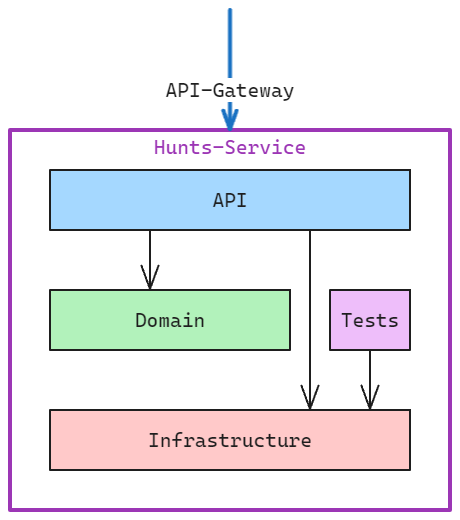
\includegraphics[width=0.6\textwidth]{images/PrAr-Software-Entwurf-Hunt-Api-Hunt-Service.png}
    \caption{Bild Hunts Microservice}
    \label{fig:swentwurf:huntapi:huntservice}
\end{figure}

Innerhalb des Hunts-Service wurde ein schichtenorientierter Ansatz gewählt, welcher Ähnlichkeiten mit der in Kapitel \ref{cha:grundlagen:swdesign:onion} beschriebenen \textit{Onion-Architecture} teilt. Jede Schicht entspricht einer horizontalen Teilung der unterschiedlichen Anwendungs-Aspekte. Für die Persistierung der Schnitzeljagden (Hunts) wurde das Repository-Pattern vorhergesehen.

Die grundlegende Funktionalität der Domäne (\textit{Hunts}, \textit{Assignments}, etc.) wird in der \textit{Domain-Schicht} zur Verfügung gestellt, welche in Abbildung \ref{fig:swentwurf:huntapi:huntservice} grün gekennzeichnet wird. Hier sind Modelle und Entities, sowie Datentypen, Enumerations und Repository-Interfaces definiert, die im System durchweg Verwendung finden. Die Domain-Schicht ist abgekapselt von Anwendungs- und Infrastrukturlogik und besitzt daher keine Abhängigkeiten zu externen Modulen.

Eine Implementierung der Repository-Interfaces wird in der \textit{Infrastruktur-Schicht} (Infrastructure) zur Verfügung gestellt, die in Abbildung \ref{fig:swentwurf:huntapi:huntservice} rot hervorgehoben wird. Diese kann zudem unabhängig von der Domänen-Logik isoliert getestet werden, wie in in Abbildung \ref{fig:swentwurf:huntapi:huntservice} lila dargestellt wird.

Die \textit{Anwendungs-Schicht} ist in Abbildung \ref{fig:swentwurf:huntapi:huntservice} blau hervorgehoben und bündelt die Funktionalität der Domain-Schicht und Infrastruktur-Schicht gemeinsam. Über eine einheitliche Schnittstelle (\textit{api/Hunt}) können Schnitzeljagden erstellt, bearbeitet, gelöscht und aufgelistet werden.

\subsubsection{Schnittstellendefinition}

\begin{figure}[H]
    \centering
    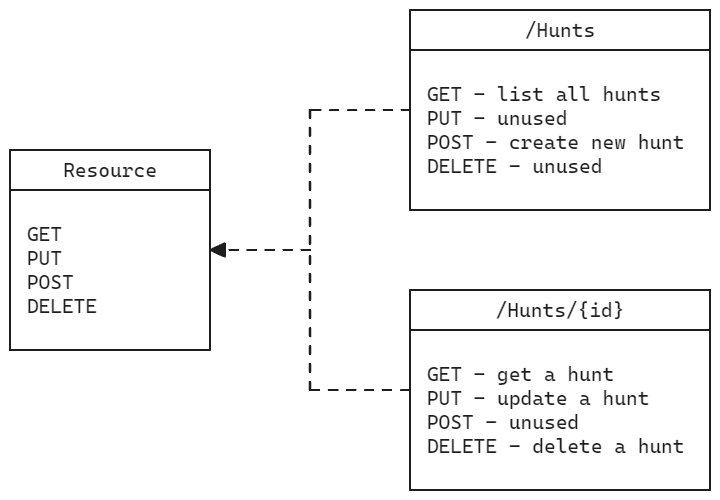
\includegraphics[width=0.6\textwidth]{images/PrAr-Software-Entwurf-Hunt-Api-Hunt-Service-Endpoints.png}
    \caption{Skizze der Hunts Ressourcenansicht}
    \label{fig:swentwurf:huntapi:huntservice:endpoints}
\end{figure}

In Abbildung \ref{fig:swentwurf:huntapi:huntservice:endpoints} sind die unterschiedlichen Operationen auf Schnitzeljagden (\textit{Hunts}) anhand des ressourcen-orientierten Ansatz aus Kapitel \ref{cha:grundlagen:collaboration:rest} dargestellt. Diese entspricht der tatsächlichen Schnittstelle, die für den Hunts-Service vorhergesehen wurde.

\subsubsection{Datenbank-Modell}

\begin{figure}[H]
    \centering
    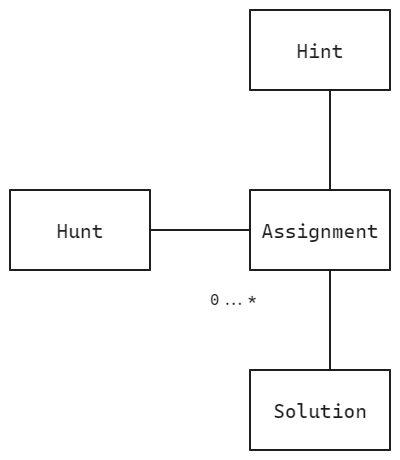
\includegraphics[width=0.6\textwidth]{images/PrAr-Software-Entwurf-Hunt-Api-Hunt-Service-Er.png}
    \caption{Skizze ER-Modell der Hunts}
    \label{fig:swentwurf:huntapi:huntservice:er}
\end{figure}

Abbildung \ref{fig:swentwurf:huntapi:huntservice:er} beschreibt das gewählte Entity-Relationship Diagram für das Datenbank-Modell des Hunts-Service.

\begin{itemize}
    \item \textbf{Hunt}: Die Schnitzeljagd. Enthält einen Titel, eine Beschreibung und eine Liste von 0 bis n Aufgaben (\textit{Assignments}).
    \item \textbf{Assignment}: Eine konkrete Aufgabe einer Schnitzeljagd. Besteht aus einem Hinweis (\textit{Hint}) und eine Lösung (\textit{Solution}).
    \item \textbf{Hint}: Ein Hinweis. Besteht aus einem Hinweis-Typ (als Enumeration) und den Hinweis-Daten als String.
    \item \textbf{Solution}: Eine Lösung zu einem gegebenen Hinweis. Besteht aus einem Lösungs-Typ (als Enumeration) und den Lösungs-Daten als String.
\end{itemize}

Wieso auf die Verwendung eines abtrakten Datenmodells verzichtet wurde, wird im Anhang \ref{appendix:adr:er} näher beschrieben.

\subsection{Participants-Service} \label{cha:swentwurf:participantsservice}

\subsubsection{Übersicht}

Damit ein Teilnehmer an einer Schnitzeljagd teilnehmen und diese auch durchführen kann, soll ihm die Anmelde- und Spielfunktionalität zur Verfügung gestellt werden. Dies wird über den Participants-Service ermöglicht. Abbildung \ref{fig:swentwurf:huntapi:participantservice} zeigt die Struktur des Dienstes.

\begin{figure}[H]
    \centering
    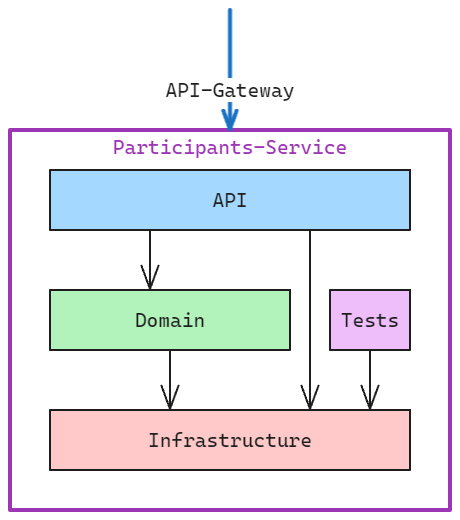
\includegraphics[width=0.6\textwidth]{images/PrAr-Software-Entwurf-Hunt-Api-Participant-Service.png}
    \caption{Bild Participants Microservice}
    \label{fig:swentwurf:huntapi:participantservice}
\end{figure}

Der Participants-Service besitzt eine ähnliche Struktur wie der Hunts-Service aus Kapitel \ref{cha:swentwurf:huntsservice} und erfüllt die Aufgabe der Teilnahmen-Verwaltung.

\subsubsection{Schnittstellendefinition}

\begin{figure}[H]
    \centering
    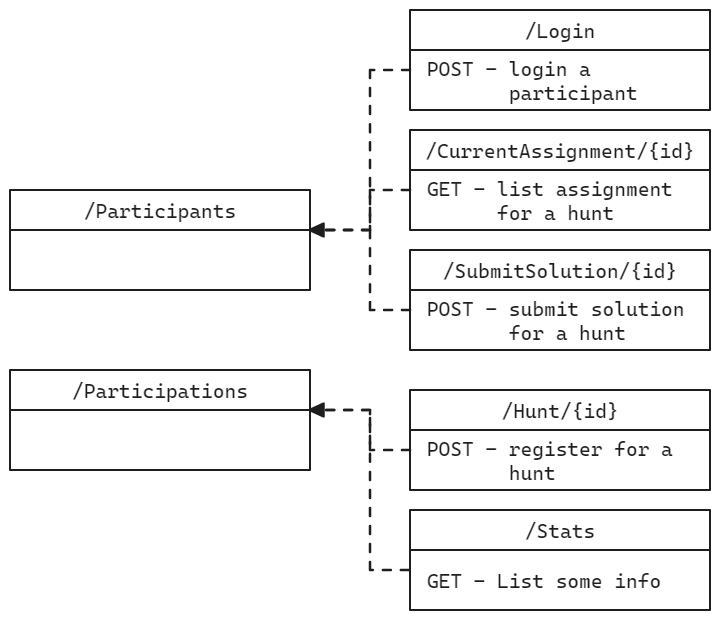
\includegraphics[width=0.6\textwidth]{images/PrAr-Software-Entwurf-Hunt-Api-Participant-Service-Endpoints.png}
    \caption{Skizze der Participants Schnittstelle}
    \label{fig:swentwurf:huntapi:participantservice:endpoints}
\end{figure}

Abbildung \ref{fig:swentwurf:huntapi:participantservice:endpoints} definiert die vorhergesehene Schnittstelle für den Participants-Service.

Unter dem Endpunkt \textit{Teilnehmer} wird dem Teilnehmer die Funktionalität zum \textit{Login} angeboten. Hierüber erhält er zusätzlich Informationen über die aktuell angemeldeten Schnitzeljagden. Möchte er eine entsprechende Schnitzeljagd starten oder fortsetzen, kann er dazu über \textit{Current-Assignment} den aktuellen Hinweis anfordern. Wenn der Teilnehmer dem Hinweis gefolgt ist und die Lösung gefunden hat, kann er diese dem System mit \textit{Submit-Solution} mitteilen. Das System stellt dann fest, ob die Lösung korrekt ist.

Der genaue Ablauf und das Zusammenspiel der einzelnen Endpunkte wird in Kapitel \ref{cha:swentwurf:spielablauf} erläutert.

Damit sich Teilnehmer für eine Schnitzeljagd anmelden können, ist unter dem Endpunkt \textit{Teilnahmen} mit \textit{Schnitzeljagd} und entsprechender \textit{Schnitzeljagd-ID} eine Registrierungsmöglichkeit vorgesehen. Zusätzlich können allgemeine Informationen wie z.B. die Anzahl der Teilnehmer oder die Anzahl aller Teilnahmen an Schnitzeljagden über den Endpunkt \textit{Stats} aufgelistet werden.

\subsubsection{Datenbank-Modell}

\begin{figure}[H]
    \centering
    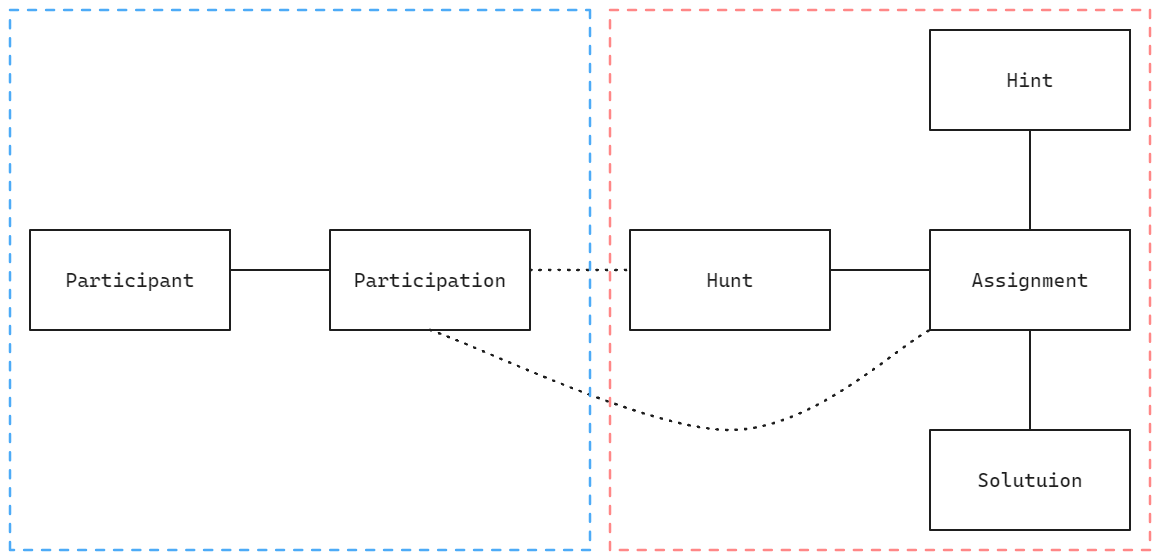
\includegraphics[width=0.6\textwidth]{images/PrAr_Software-Entwurf-Hunt-Api-Participant-Service-Er.png}
    \caption{Skizze ER-Modell zwischen Hunts und Participants}
    \label{fig:swentwurf:huntapi:participantservice:er}
\end{figure}

Abbildung \ref{fig:swentwurf:huntapi:participantservice:er} beschreibt das gewählte Entity-Relationship-Diagramm für das Datenbankmodell des Participants-Service. Die Teilnahmen (Participants und Participations) sollen relational gespeichert werden, während die Schnitzeljagden in einem nicht-relationalen Modell (z.B. Redis-Cache) gespeichert werden sollen, da diese bereits korrekt im Hunts-Service gespeichert werden (siehe Kapitel \ref{cha:swentwurf:huntsservice}).
